%% PRE EDITION
\documentclass[a4paper]{article}
%\documentclass[border=5pt]{standalone} % Border allows to adjust the white space around the figure
\usepackage[utf8]{inputenc}
\usepackage[T1]{fontenc}
\usepackage[francais,english]{babel}
\usepackage{soul}
\usepackage[pdftex]{graphicx}
\usepackage{geometry}
\geometry{hmargin=3cm,vmargin=2.5cm}
\usepackage{tabularx}
\usepackage{multirow}
\usepackage{float}
\usepackage{xcolor}


% Tikz - Pgfplot
% ========================================================================
\usepackage{tikz}
\usepackage{pgfplots}
\pgfplotsset{compat=newest}
\usetikzlibrary{shapes,arrows,shadows,patterns,pgfplots.groupplots,decorations.markings,chains}
\usetikzlibrary{positioning}

% AlgoPackage
% ========================================================================
% \usepackage{times}
% \usepackage[ruled,vlined]{algorithm2e}
% \include{pythonlisting}
\usepackage{algorithm}
\usepackage[noend]{algpseudocode}


% Ref package
% ========================================================================
\usepackage{hyperref}
\usepackage{authblk}


% Symbols
% ========================================================================
\usepackage{amsfonts}
\usepackage{amsmath}
\usepackage{amssymb}
\usepackage{mathrsfs}
\usepackage{booktabs}
\usepackage{siunitx}
\usepackage{ulem}

% Theorem
% ========================================================================
\usepackage{amsthm}
\usepackage{thmtools}
\newenvironment{remarque}{\textbf{Remarque:}}{}

% ========================================================================
\title{Optimisation bi-convexe}
\author{Cecile Della Valle}

%% DEBUT DE REDACTION
\begin{document}

\maketitle

%%%%%%%%%%%%%%%%%%%%%%%%%%%%%%%%%%%%%%%%%%%%%%%%%%%%%%%%%%%%%%%%%%%%%%%%%%%%%%%%%%%%%%%%%%%%%%%%%%%%%%%%%%%%%%%%%%%%%%%%%%%%%%%%%
%%%%%%%%%%%%%%%%%%%%%%%%%%%%%%%%%%%%%%%%%%%%%%%%%%%%%%%%%%%%%%%%%%%%%%%%%%%%%%%%%%%%%%%%%%%%%%%%%%%%%%%%%%%%%%%%%%%%%%%%%%%%%%%%%
%%%%%%%%%%%%%%%%%%%%%%%%%%%%%%%%%%%%%%%%%%%%%%%%%%%%%%%%%%%%%%%%%%%%%%%%%%%%%%%%%%%%%%%%%%%%%%%%%%%%%%%%%%%%%%%%%%%%%%%%%%%%%%%%%
%%%%%%%%%%%%%%%%%%%%%%%%%%%%%%%%%%%%%%%%%%%%%%%%%%%%%%%%%%%%%%%%%%%%%%%%%%%%%%%%%%%%%%%%%%%%%%%%%%%%%%%%%%%%%%%%%%%%%%%%%%%%%%%%%


%%%%%%%%%%%%%%%%%%%%%%%%%%%%%%%%%%%%%%%%%%%%%%%%%%%%%%%%%%%%%%%%%%%%%%%%%%%%%%%%%%%%%%%%%%%%%%%%%%%%%%%%%%%%%%%%%%%%%%%%%%%%%%%%%
\section*{Introduction}
%%%%%%%%%%%%%%%%%%%%%%%%%%%%%%%%%%%%%%%%%%%%%%%%%%%%%%%%%%%%%%%%%%%%%%%%%%%%%%%%%%%%%%%%%%%%%%%%%%%%%%%%%%%%%%%%%%%%%%%%
On introduit le probleme d'optimisation biconvex-concave
de déconvolution aveugle d'images 
avec l' a priori de noyau de convolution régulier,
\[
\underset{u \in U ,K \in \Sigma}{\text{min}} \; \underset{v}{\text{sup}} \;
\frac{1}{2} \| g - K * u\|^2 
+ \frac{1}{2} \alpha \| D K \|^2
+ \langle \nabla u , v \rangle
- \chi_{B,\mu}(v)
\; .
\]
L'espace $\Sigma$ correspond à l'ensemble des simplexes 
(ensemble des noyaux à coefficient positif dont la somme des coefficients vaut 1).
Par extension on notera $\Sigma$ la fonction indicatrice de cet ensemble.
L'espace $U$ correspond à l'hypercube $[0,1]^{N_x \times N_y}$, ou la boule unité pour la norme $L^\infty$.
Sa fonction indicatrice correspond donc à $\chi_{B,1}$.
La fonction à minimiser peut alors se réécrire
\[
\underset{u ,K }{\text{min}} \; \underset{v}{\text{sup}} \;
\frac{1}{2} \| g - K * u\|^2 
+ \chi_{B,1} (u)
+ \frac{1}{2} \alpha \| D K \|^2
+ \Sigma(K)
+\langle \nabla u , v \rangle
- \chi_{B,\mu}(v)
\; .
\]
On note
\[
L(u,v,K)
 =\frac{1}{2} \| g - K * u\|^2 
+ \frac{1}{2} \alpha \| D K \|^2
+ \langle \nabla u , v \rangle
- \chi_{B,\mu}(v)
\]
On souhaite comparer deux stratégies pour résoudre ce problème :
\begin{itemize}
    \item Minimisation alternée : on scinde la fonction à minimiser en une partie qui dépend de l'image $u$ 
    et une partie qui dépend du noyau $K$, les deux fonctions sont minimisées jusqu'à convergence, alternativement.
    \item Minimisation par pas de descente alterné (PDA) : l'algorithme alterne les pas de descente entre l'image $u$, le noyau $K$ et la variable auxiliaire (ou duale) $v$.
\end{itemize}
Pour chacune de ces deux méthodes, on effectue les trois tests suivants :
\begin{itemize}
     \item Initialisation par le noyau exacte, bruit std = $0.05$, $(\alpha,\mu) = (1,5)$  (cas 1);
     \item Initialisation par un noyau approché, pas de bruit, $(\alpha,\mu) = (1,5)$  (cas 2) ;
      \item Initialisation par un noyau approché, bruit std = $0.05$, $(\alpha,\mu) = (1,5)$  (cas 3) ;
\end{itemize}
On fixe les paramètres $(\alpha,\mu)$ pour toutes les expériences, même s'ils ne sont pas optimaux en terme de reconstruction. 
Ce qui nous intéresse ici c'est seulement la convergence des algorithmes.

\begin{remarque}
J'ai retiré la projection sur Simplex finalement car les algorithmes ne marchaient pas bien. 
En fait le résultat de la projection donnait des noyaux irréguliers.
A la place j'ai projeté sur un hypercube avec une valeur max et une valeur min, cela avait l'avantage d'être simple à implémenter, d'avoir un bon comportement et de rester cohérent avec le problème initial (?).
\end{remarque}

%%%%%%%%%%%%%%%%%%%%%%%%%%%%%%%%%%%%%%%%%%%%%%%%%%%%%%%%%
\section{Minimisation alternée}

On introduit les deux sous problèmes suivants :

\begin{align}
E_1(K) = \frac{1}{2} \| g - K * u\|^2 + \frac{1}{2} \alpha \| D K \|^2 + \Sigma(K) \\
E_2(u) = \frac{1}{2} \| g - K * u\|^2 +  \mu \text{TV} (u)
\end{align}

Dans la minimisation alternée, on considere d'abord la minimisation de $E_2$ 
pour reconstruire l'image $u$. 
La minimisation est obtenur par un algorithme de Chambolle-Pock.
 Puis on minimise $E_1$ pour reconstruire le noyau $K$ avec un forward-backward.
On alterne 5 fois entre chaque minimisation, chacune a 200 pas d'itérations, donc en fait on est pas complètement à convergence..



%%%%%%%%%%%%%%%%%%%%%%%%%%%%%%%%%%%%%%%%%%%%%%%%%%%%%%%%%
\section{Pas de descente alterné (PDA)}
%


Pour résoudre ce probleme d'optimisation on se propose de tester l'algorithme suivant,
\begin{align}
& K_{k+1} = \text{prox}_{\Sigma} \; (K_k - \gamma \partial_K L(u_k,K_k,v_k) \; )\\
& u_{k+1} = \text{proj}_{B_1} \; (u_k - \tau \partial_u L(u_k,K_{k+1},v_k) \; )\\
& v_{k+1}         = \text{prox}_{B_\mu} \; (v_k + \sigma \partial_v L (\bar{u}_k,K_{k+1},v_k) \; )\\
&\bar{u}_{k+1} = u_{k+1} + \theta (u_{k+1} - u_k) \quad \text{(relaxation)}
\end{align}
On écrit alors les dérivées partielles de $L$,
\begin{align}
& \partial_K L(u_k,K_k,v_k) \; ) = - (g-K_k*u_k)*\tilde{u}_k+ \alpha D^TDK_k \\
& \partial_u L(u_k,K_{k+1},v_k) \; ) = \text{div} \cdot v_k - \tilde{K}_k * (g-K_k*u_k)\\
& \partial_v L (\bar{u}_k,K_{k+1},v_k) \; ) =  \nabla \bar{u}_k
\end{align}
Pour les opérateurs $\nabla$ et $\div$ j'ai repris les opérateurs discrets du docuement 120415-deconvolution que tu avais écrit.

On trace les énergies primales et duales au cours de la minimisation

\begin{align}
& Ep_K = \frac{1}{2} \| g - K * u\|^2 
+ \frac{1}{2} \alpha \| D K \|^2\\
& Ep_x = \frac{1}{2} \| g - K * u\|^2 
+ \mu. \text{TV} (u)  \\
& Ed = - \langle \nabla u ,v \rangle 
\end{align}

L'algorithme est très sensible aux pas de descente choisi.
Soit $\ell_1$ le coefficient de Lipshitz de $E_1$, le pas de descente pour le noyau $K$
est choisi par
\[
\tau = c \cdot \frac{2}{\ell_1} \leq  c \cdot \frac{1}{\|u\|^2 + \alpha \|D\|^2} \quad 0<c \leq 1 \; .
\]
En effet on ne veut pas dépasser la valeur limite du pas de descente pour assurer la convergence de la descente de gradient, mais on ne veut pas nécessairement effectuer un pas optimal non plus, par exemple si le noyau est initialisé de façon exacte.
On choisit donc la stratégie suivante, à chaque pas de temps le coeffecient $c$ est multiplié par $0.98$. La valeur initiale est ajustée à la main. Cela permet notamment de choisir un $c$ supérieur a $1$. En effet j'ai choisi cette stratégie quand le noyau est très peu modifié par rapport à l'image, cela améliore nettement la convergence.
Pour le pas de descente de l'image et de la variable auxilière cette fois, on respecte la condition de convergence de Chambolle-Pock
\[
\sigma_u \sigma_v <\frac{1}{L^2} \leq \left(\frac{1}{\sqrt{8} + \| k \|^2} \right)^2
\; .
\]
J'ai testé plusieurs stratégies, mais mettre le pas "optimal" marchait mieux jusqu'à présent.

\section{Figures}

%
\begin{figure}[h]
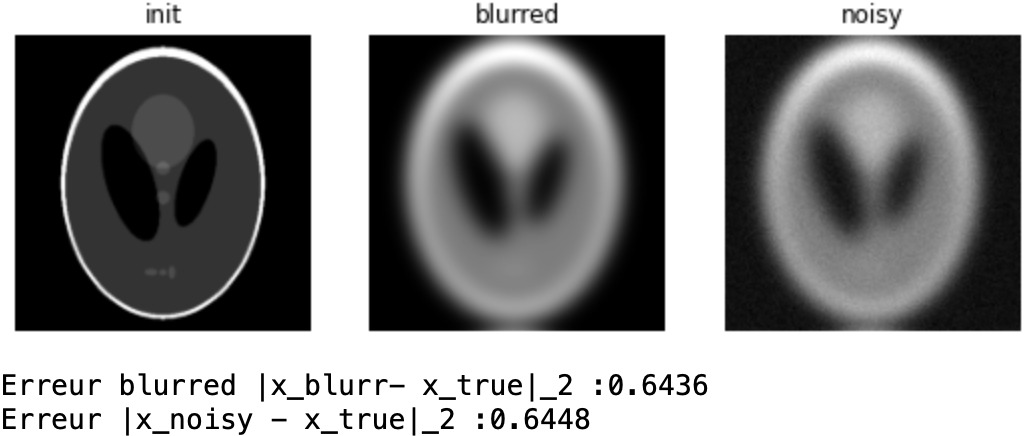
\includegraphics[scale=0.6]{figures/shepp-logan}
\caption{Image utilitée pour la reconstruction, image convoluée et image bruitée convoluée.}
\end{figure}
%
\begin{figure}[h]
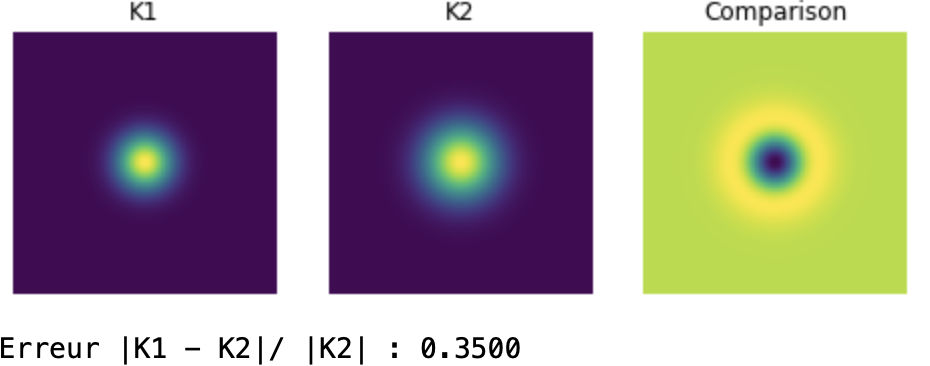
\includegraphics[scale=0.6]{figures/kernel}
\caption{Le noyau exact K1 et un noyau proche K2 pour l'initialisation de l'algorithme (de même centre mais un peu plus large).
L'erreur initiale sur le noyau s'élève donc à environ $28\%$.}
\end{figure}

\begin{figure}[h]
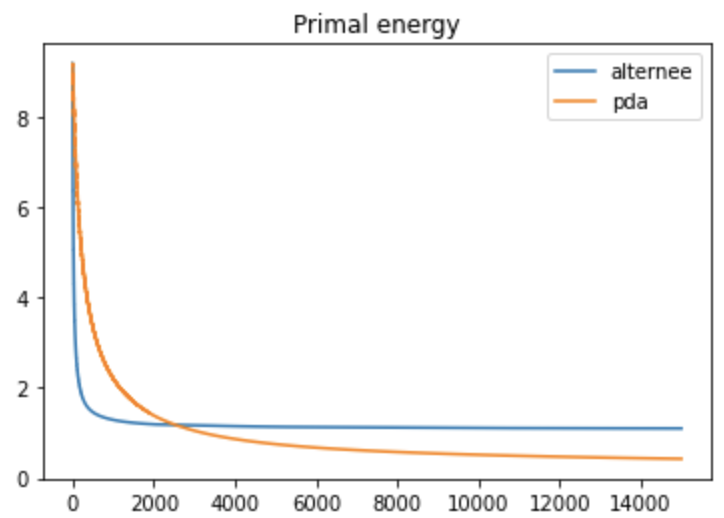
\includegraphics[scale=1.0]{figures/cas1}	
\caption{(cas1)  initialisation du noyau $K$ exact, bruit std =0.05.}
\end{figure}
%
\begin{figure}[h]
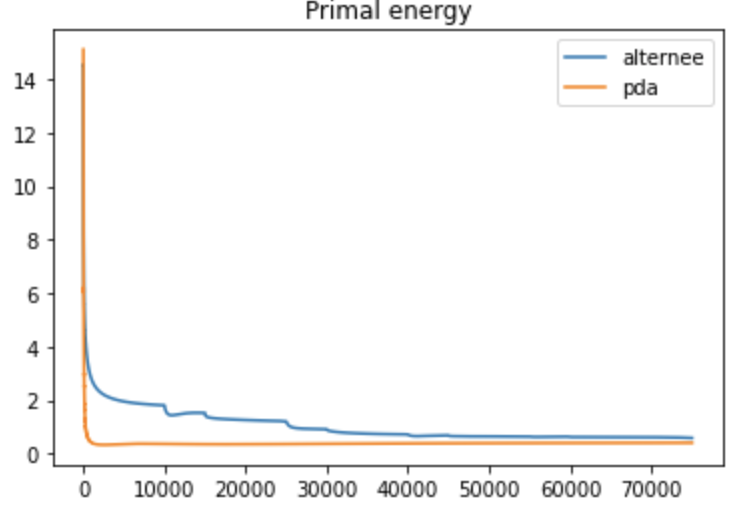
\includegraphics[scale=1.0]{figures/cas2}	
\caption{(cas2)  initialisation du noyau approché, pas de bruit}
\end{figure}
%
\begin{figure}[h]
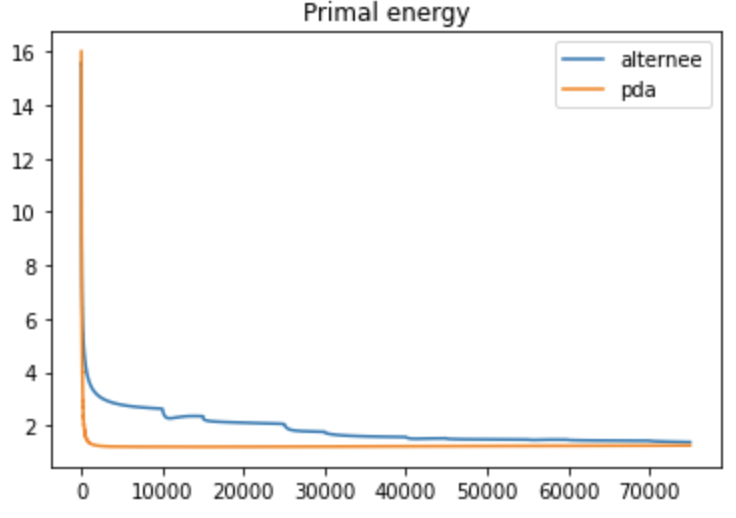
\includegraphics[scale=1.0]{figures/cas3}	
\caption{(cas3) initialisation du noyau approché, bruit std =0.05}
\end{figure}
%
\begin{figure}[h]
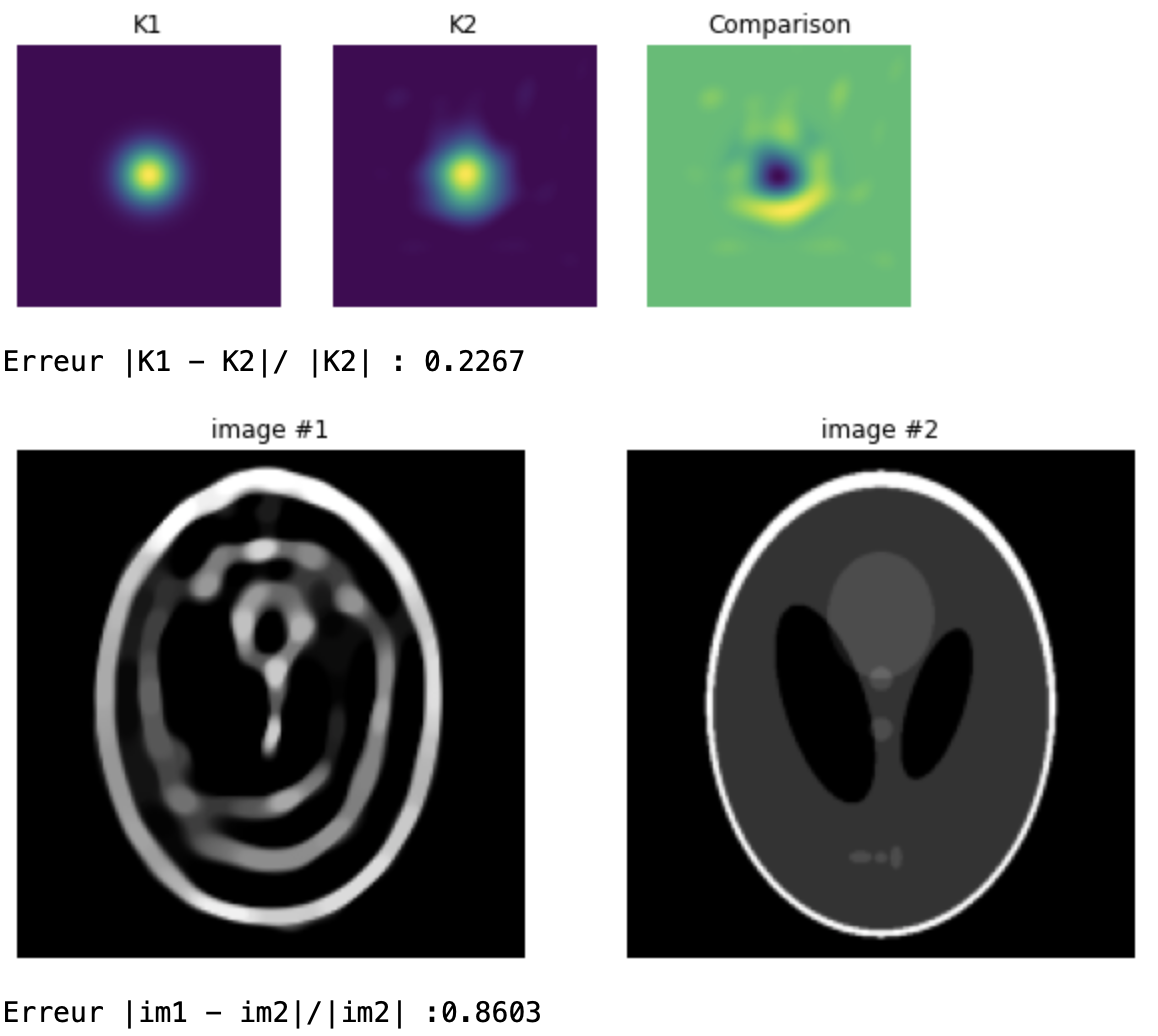
\includegraphics[scale=0.6]{figures/altrn-cas2}	
\caption{Reconstruction pour la minimisation alternée pour le cas 2.}
\end{figure}
%
\begin{figure}[h]
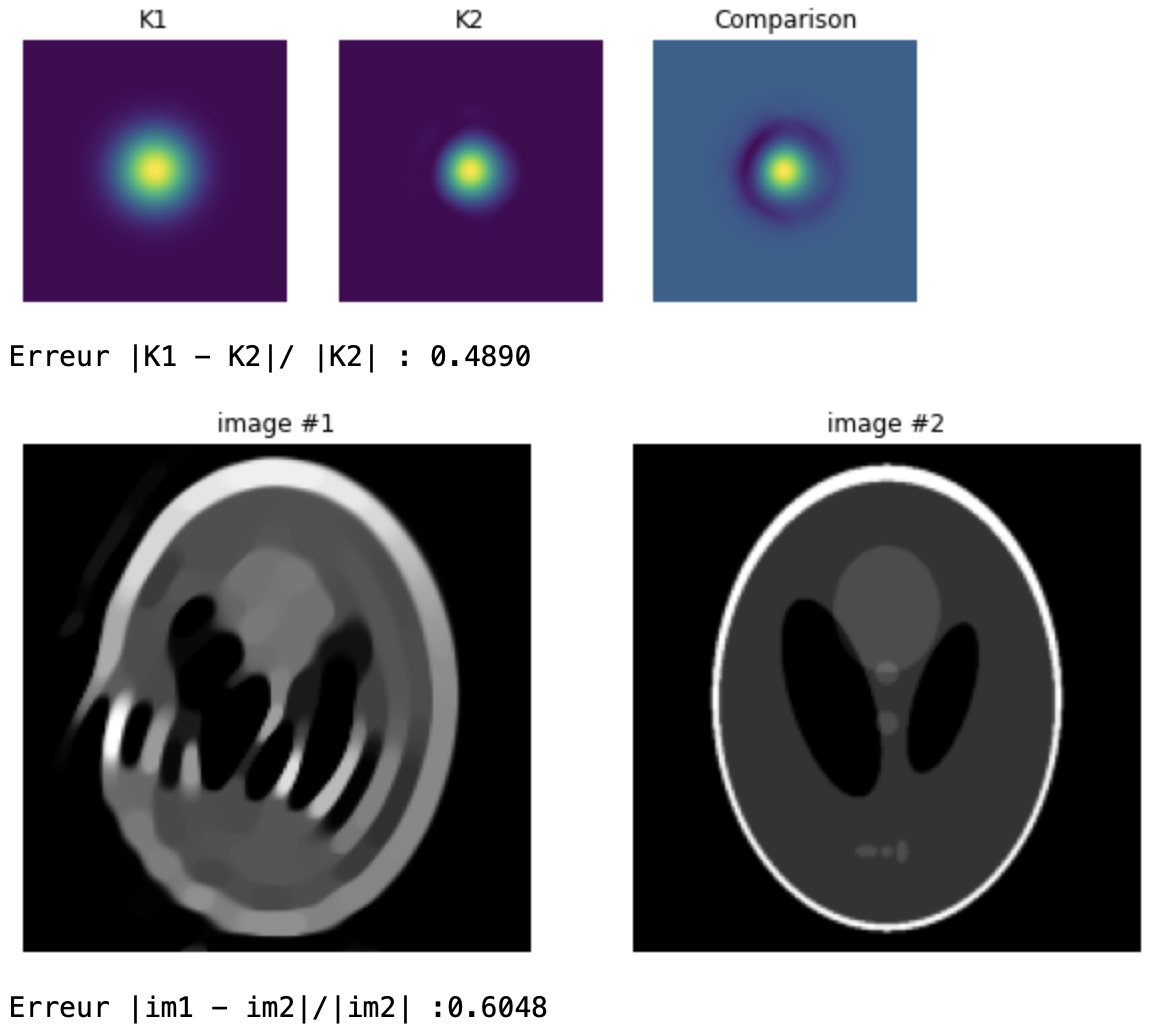
\includegraphics[scale=0.6]{figures/pda-cas2}	
\caption{Reconstruction pour la minimisation par pas de descente altermé pour le cas 2.}
\end{figure}
%
%
\begin{figure}[h]
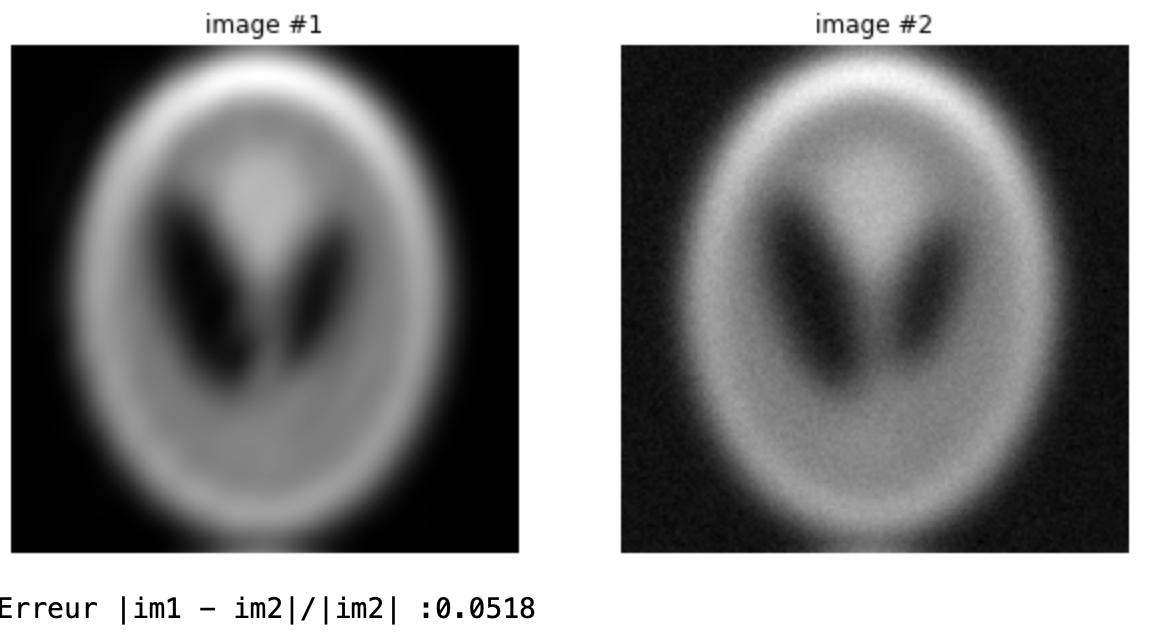
\includegraphics[scale=0.6]{figures/convolve-cas2}	
\caption{Comparaison des images convoluées pour le cas 3 par pas de descente alternée. A gauche la convolution entre l'image et le noyau issus de la minimisation a droite l'image bruitée donnée en entrée de l'algorithme. La différence (ou erreur de reconstruction) est comparable au bruit.}
\end{figure}
%
%%%%%%%%%%%%%%%%%%%%%%%%%%%%%%%%%%%%%%%%%%%%%%%%%%%%%%%%%%%%%%%%%%%%%%%%%%%%%%%%%%%%%%%%%%%%%%%%%%%%%%%%%%%%%%%%%%%%%%%%%%%%%%%%%
%%%%%%%%%%%%%%%%%%%%%%%%%%%%%%%%%%%%%%%%%%%%%%%%%%%%%%%%%%%%%%%%%%%%%%%%%%%%%%%%%%%%%%%%%%%%%%%%%%%%%%%%%%%%%%%%%%%%%%%%%%%%%%%%%
%%%%%%%%%%%%%%%%%%%%%%%%%%%%%%%%%%%%%%%%%%%%%%%%%%%%%%%%%%%%%%%%%%%%%%%%%%%%%%%%%%%%%%%%%%%%%%%%%%%%%%%%%%%%%%%%%%%%%%%%%%%%%%%%%
%%%%%%%%%%%%%%%%%%%%%%%%%%%%%%%%%%%%%%%%%%%%%%%%%%%%%%%%%%%%%%%%%%%%%%%%%%%%%%%%%%%%%%%%%%%%%%%%%%%%%%%%%%%%%%%%%%%%%%%%%%%%%%%%
\end{document}

